\documentclass{article}

% import packages
\usepackage[utf8]{inputenc}
\usepackage{graphicx}
\usepackage{geometry}
\usepackage{amsmath}
\usepackage{bm}
\usepackage{amsfonts}
\usepackage{amssymb}
\usepackage{dsfont}
\usepackage{float}
\usepackage{caption}
\usepackage{subcaption}
\usepackage{enumitem}
\usepackage{hyperref}
\usepackage{cancel}
\usepackage{pifont}
\usepackage{pdfpages}
\usepackage{comment}
\usepackage{hanging}
% \usepackage{gensymb}
\usepackage{textcomp}
\usepackage{natbib}

% define commands
\newcommand{\dai}[2]{\frac{\partial #1}{\partial #2}}
\newcommand{\deriv}[2]{\frac{\mathrm{d} #1}{\mathrm{d} #2}}
\newcommand{\Deriv}[2]{\frac{\mathrm{D} #1}{\mathrm{D} #2}}
\newcommand{\R}{\mathds{R}}
\newcommand{\C}{\mathds{C}}
\newcommand{\Z}{\mathds{Z}}
\newcommand{\N}{\mathds{N}}
\newcommand{\bigo}{\mathcal{O}}
\newcommand{\eps}{\varepsilon}
\newcommand{\curl}{\nabla\times}
\newcommand{\dd}{\mathrm{d}}
\newcommand{\uvec}[1]{\mathbf{\hat{#1}}}
\DeclareMathOperator{\sgn}{sgn}
\DeclareMathOperator{\sinc}{sinc}
\DeclareMathOperator{\sech}{sech}
\DeclareMathOperator{\csch}{csch}
\renewcommand{\Re}{\text{Re}}
\renewcommand{\Im}{\text{Im}}
\newcommand{\cmark}{\ding{51}}%
\newcommand{\xmark}{\ding{55}}%
\newcommand{\qqquad}{\qquad\qquad}


\geometry{left=25mm, top=25mm, right=25mm, bottom=25mm}
\title{Graduate Student Researcher salaries at Scripps Institution of Oceanography, 2015--2025}
\author{Hayden A. Johnson}
\date{\today}

\begin{document}

\maketitle

\section{Introduction}

When I started as a PhD student at Scripps Institution of Oceanography (SIO) in September of 2019, my salary as a Graduate Student Researcher (GSR) was \$32,000. Over the past four and a half years, it has increased to over \$40,000, and is expected to settle at a little over \$43,000 by October of 2024. The initial portion of this increase was a result of raises given voluntarily by the SIO department, while the latter portion has been a result of raises mandated by the recently negotiated GSR contract.

Over the same time period, the cost of living has also increased rapidly, driven by a once-in-a-century plague and a chronic housing shortage. Inflation hit levels not seen for decades, and rent has risen both off- and on-campus. At a glance, it is therefore difficult to tell what the net result of these two competing effects has been.

This report has two goals. First, I hope that it will help to explain the current situation regarding GSR salaries at SIO, and the history of how things came to be the way they are. Second, it is an incomplete attempt to come up with a quantitative answer to the question of whether increases in GSR salaries have exceeded, kept up with, or fallen behind increases in the cost of living in San Diego in recent years.

\section{GSR salaries over time}

Salaries of SIO GSRs have been increasing somewhat steadily over the duration of the available record of salary information. The way in which GSR salaries are determined changed dramatically with the collectively-bargained GSR contract signed in December of 2022, and it is useful to draw a delineation between the pre- and post-contract eras. Salary information during each of these eras is outlined in the two sections below.

\subsection{Prior to collectively bargained contract}

Prior to the collectively bargained contract signed in December of 2022, GSR salaries were in practice set by the department, with occasional raises occurring at the department's discretion. SIO students were at the highest step, Step 10, on the old pay scale. The appointment percentage, or ``percent effort''---nominally, the fraction of time that GSRs spend as ``workers'' rather than as ``students''---was around 40\%, and was varied up or down in order to decouple changes in SIO GSR salary from changes in the GSR pay scale set by the University of California (UC), and to achieve the \$1,000 raise for advancing to candidacy. The historical SIO GSR salaries prior to the collectively bargained contract are listed in Table \ref{tab:pre_contract}.

\begin{table}[h]
	\centering
	\caption{Historical annual salaries of GSRs at SIO in US Dollars. Data from July 2014 to August 2019 were obtained from \cite{kachelein} (personal communication). Data from September 2019 to the present were obtained from my own personal financial records, and emails received from the department detailing changes to GSR pay.}
	\label{tab:pre_contract}
	\begin{tabular}{l r r}
		\hline		
		Start date & Pre-qualification & Post-qualification \\
		\hline
		2014-07-01 & 30,000.00 & 31,000.00 \\
		2019-07-01 & 32,000.00 & 33,000.00 \\
		2021-07-01 & 33,000.00 & 34,000.00 \\
		2022-07-01 & 34,000.00 & 35,000.00 \\
		\hline
	\end{tabular}
\end{table}

\subsection{Collectively bargained contract}

As a result of the unionization of GSRs under the United Auto Workers (UAW) umbrella, and the subsequent GSR strike in November--December of 2022, the University and the Union agreed to a new contract for GSRs (available here: \citep{gsr_contract}). It was signed in December of 2022 and the wages article took effect on April 1$^\text{st}$, 2023. The new contract has only six pay scale steps, and it is clearly specified that GSRs at Step 10 on the old pay scale must move to Step 6 on the new pay scale. It is also clearly specified that individual students can have their pay scale step increased but never decreased. All GSRs at SIO who were enrolled prior to April 1$^\text{st}$, 2023 (referred to here as ``Old Students'') are therefore required to be at Step 6 of the new pay scale.

The Union's interpretation of the GSR contract is that it also implies that GSRs should be appointed at 50\% effort. Though UC has disagreed with this, students at SIO who started after April 1$^\text{st}$, 2023 (referred to here as ``New Students'') have been appointed at 50\% of Step 3 or Step 4, pre- or post-qualification. Old Students at SIO have been appointed at 40\% or 43\%, pre- or post-qualification, since the new contract took effect, with those percentages chosen to match the salaries of Old and New students as closely as possible \citep{salary_implementation_email}.

The Union filed a grievance against UC claiming that sub-50\% appointments for GSRs are a violation of the GSR contract. In a settlement agreed to by the Union and the University on January 26$^\text{th}$, all GSRs with appointments in the rage of 40--49\% will be moved to 50\% effective April 1$^\text{st}$, 2024 \citep{uc_uaw_page}. According to the University, this change in appointment percentage will be temporary and last only for the duration of Spring Quarter \citep{uc_uaw_page}. As a result of this temporary pay increase, Old Students who are paid as GSRs will receive a net total of \$1,651.90 or \$2,359.80, pre- or post-qualification. Old Students with fellowships will not have their appointment percentages adjusted, but will instead receive a lump-sum payment of \$1,000 \citep{uc_uaw_page}. New Students are already appointed at 50\%, and their salaries will therefore be unaffected by this settlement. The Union has filed a separate grievance claiming that the University cannot appoint incoming students at a lower step than existing students; this grievance has progressed to arbitration and is expected to be ruled on in several months.

The step, percentage appointment, and resulting salary for New and Old Students, pre- and post-qualification, over the duration of the contract are listed in Table \ref{tab:contract}. Note that the post-qualification pay for New Students is included here for the sake of completeness, but it is of little practical consequence, because it is unlikely that any new students will advance to candidacy before the expiration of the current contract on May 31$^\text{st}$, 2025.

\begin{table}[h]
	\centering
	\caption{Historical and expected annual salaries of GSRs at SIO in US Dollars. These salaries are determined based on the implementation of the wages article of the contract signed between the Student Researchers Union and the University of California in December of 2023, which took effect April 1$^\text{st}$, 2023, and the settlement of the 50\% appointment grievance, which is expected to take effect April 1$^\text{st}$, 2024. The source of this information is the \cite{gsr_contract}, the \cite{salary_implementation_email}, and the \cite{uc_uaw_page}.}
	\label{tab:contract}
	\begin{tabular}{l r r r r r r r r r r r r}
		\hline		
		& \multicolumn{6}{c}{New Students} & \multicolumn{6}{c}{Old Students} \\
		& \multicolumn{3}{c}{Pre-qualification} & \multicolumn{3}{c}{Post-qualification} & \multicolumn{3}{c}{Pre-qualification} & \multicolumn{3}{c}{Post-qualification} \\
		\hline
		Start date & Step & \% & Salary & Step & \% & Salary & Step & \% & Salary & Step & \% & Salary \\
		\hline
		2023-04-01 & 3 & 50 & 35,457.50 & 4 & 50 & 38,205.50 & 6 & 40 & 35,485.60 & 6 & 43 & 38,147.02 \\
		2023-10-01 & 3 & 50 & 37,727.00 & 4 & 50 & 40,651.00 & 6 & 40 & 37,756.80 & 6 & 43 & 40,588.56 \\
		2024-04-01 & 3 & 50 & 37,727.00 & 4 & 50 & 40,651.00 & 6 & 50 & 47,196.00 & 6 & 50 & 47,196.00 \\
		2024-07-01 & 3 & 50 & 37,727.00 & 4 & 50 & 40,651.00 & 6 & 40 & 37,756.80 & 6 & 43 & 40,588.56 \\
		2024-10-01 & 3 & 50 & 40,130.00 & 4 & 50 & 43,240.50 & 6 & 40 & 40,162.40 & 6 & 43 & 43,174.58 \\
		\hline
	\end{tabular}
\end{table}

\section{Methods}

\label{sec:methods}

While GSR salaries at SIO have been increasing, so too has the cost of living. What matters to students more than the dollar value of salary increases is changes in salary relative to changes in the cost of living. This report attempts to quantify this using two metrics; one describing inflation, and the other describing changes in the housing rental market.

\subsection{Adjusting for inflation}

The Consumer Price Index (CPI) is compiled by the United States Bureau of Labor Statistics (BLS), and is widely used as a measure of inflation. It represents the cost of a weighted average of various consumer goods and services relative to the cost for the same goods and services at a previous point in time. A more detailed explanation is available on the BLS website \citep{cpi_overview}. For this report, the CPI for All Urban Consumers in the West Census Region is used; the data is available online from the BLS \citep{cpi_data}.

Equation \ref{eq:inflation_normalized_salary} defines an inflation-adjusted normalized salary $S_I$. In this equation, $S(t)$ is the GSR salary in USD at time $t$, and $C(t)$ is the value of the CPI at time $t$. $S_I$ is a dimensionless quantity, which represents the inflation-adjusted salary of GSRs, normalized such that the value of $S_I$ is unity at the reference time $t_0$.

\begin{equation}
	S_I(t) = \frac{S(t)/S(t_0)}{C(t)/C(t_0)}
	\label{eq:inflation_normalized_salary}
\end{equation}

Intuitively, if salary increases perfectly match inflation (as measured by the CPI), then the inflation-adjusted normalized salary $S_I$ will remain constant. If salary increases outpace inflation then $S_I$ will increase over time. Conversely, if salary increases do not keep up with inflation, then $S_I$ will decrease over time.

\subsection{Adjusting for changes in the housing rental market}

The housing rental market can be volatile and highly localized, which makes it difficult find high-quality data. The best source of data that I have been able to find is the online real-estate and rental company Zillow, which produces publicly available rental price data that can be downloaded from their website \citep{zori_data}. The Zillow Observed Rent Index (ZORI) is a weighted average of rental prices across various types of housing stock; a more detailed description is available on the Zillow website \citep{zori_overview}. For this report, the specific index used is the ZORI (Smoothed): All Homes Plus Multifamily Time Series, for the city of San Diego.

Rent-adjusted normalized salary $S_R$ is defined in Equation \ref{eq:rent_normalized_salary}, in exact analogy to the inflation-adjusted salary specified by Equation \ref{eq:inflation_normalized_salary}. $S(t)$ is the GSR salary in USD at time $t$, and $Z(t)$ is the value of the ZORI at time $t$. $S_R$ is dimensionless, with value unity at the reference time $t_0$.

\begin{equation}
	S_R(t) = \frac{S(t)/S(t_0)}{Z(t)/Z(t_0)}
	\label{eq:rent_normalized_salary}
\end{equation}

As with the inflation-adjusted normalized salary, the rent-adjusted normalized salary $S_R$ will remain constant if proportional changes in salary match proportional changes in average rent (as measured by the ZORI). If salary increases faster than average rent, then $S_R$ will increase over time. Conversely, if salary increases do not keep up with increases in rent, then $S_R$ will decrease over time.

\section{Results and discussion}

While they are far from perfect metrics, the inflation-adjusted and rent-adjusted normalized salaries $S_I$ and $S_R$ defined in Section \ref{sec:methods} can be used to better understand changes in SIO GSR salary in the context of changes in the cost of living. The value of these quantities over time is plotted in Figure \ref{fig:normalized_salaries} (a) and (b), respectively. For the sake of ease of comparison between $S_I$ and $S_R$, the reference time $t_0$ for both quantities is taken to be January 1$^\text{st}$, 2015, because that is the earliest date for which ZORI data is available.

\begin{figure}[H]
	\centering
	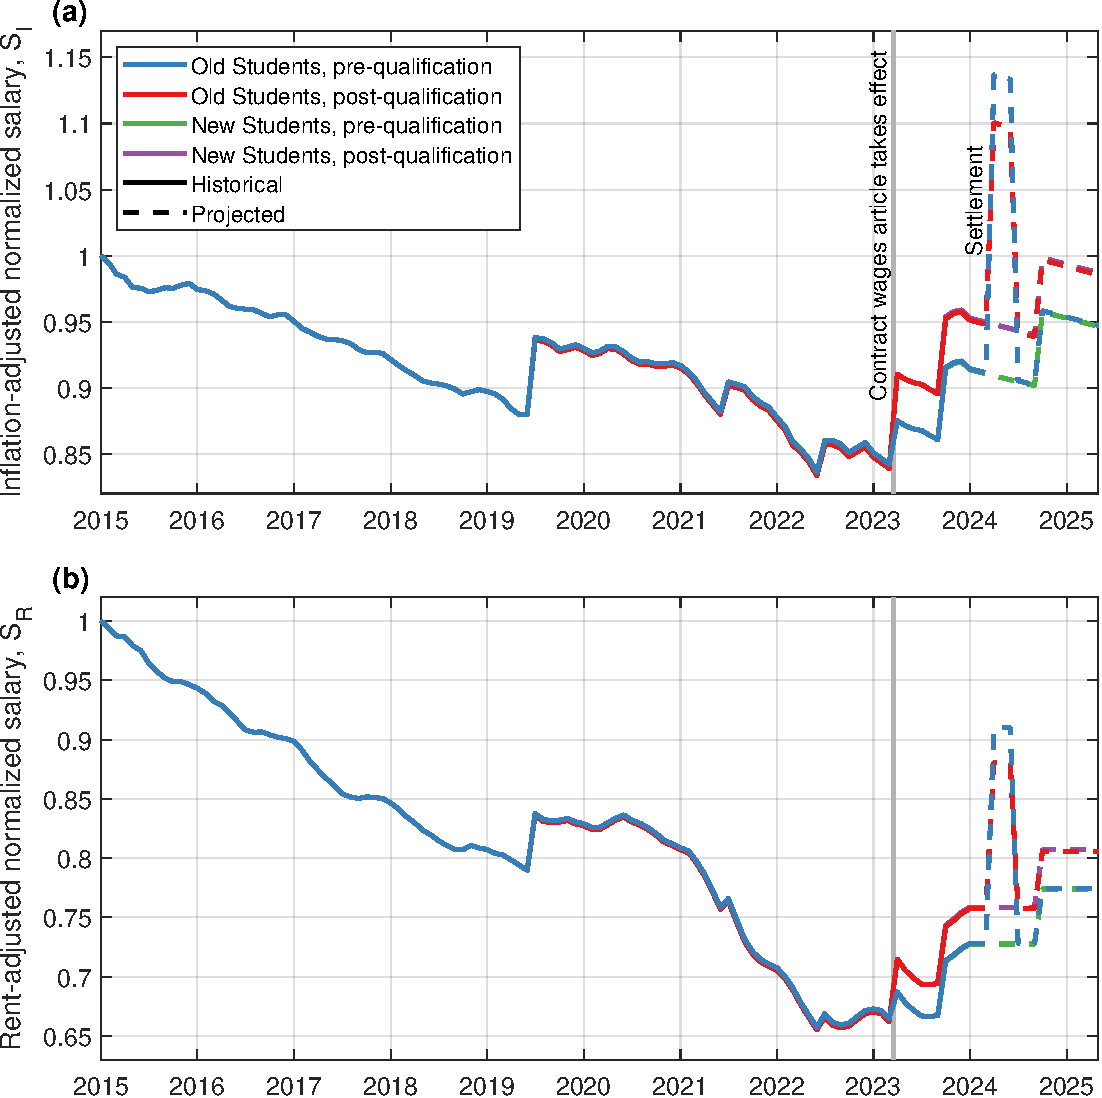
\includegraphics[width=\linewidth]{../combined_normalized_gsr_salary.pdf}
	\caption{\textbf{(a)} Inflation-adjusted and \textbf{(b)} rent-adjusted normalized salaries of GSRs at SIO from January 2015 to May 2025. The pre- and post-qualification salaries are separately normalized relative to their own respective values in January 2015. The solid lines denote historical values, and dotted lines indicate projections, assuming 2\% annual inflation for \textbf{(a)}, and that rent remains constant for \textbf{(b)}. The grey vertical line indicates the time at which the wages article of the new GSR contract took effect. The 3-month long bump in Old Student salaries is the outcome of the settlement of the appointment percentage grievance.}
	\label{fig:normalized_salaries}
\end{figure}

Despite the salary increases in July of 2019, 2021, and 2022, the period prior to the implementation of the collectively bargained GSR contract is generally defined by a decrease in the inflation- and rent-adjusted salaries $S_I$ and $S_R$. By the summer of 2022, the inflation-adjusted normalized salary had fallen to about 0.85, indicating that, accounting for inflation, SIO GSRs had actually seen a 15\% decrease in the purchasing power of their wages compared to January of 2015. The decline in the rent-adjusted normalized salary was even more pronounced, falling to about 0.67. A decrease in $S_R$ of 33\% indicates that the increase in average San Diego rent over this period was 49\% greater (1/0.67=1.49) than the increase in SIO GSR salaries. (Note that the slight separation of pre- and post-qualification normalized salaries over this period is a result of the fact that a flat dollar-amount raise represents a slightly smaller fractional increase for qualified GSRs, because their initial salary was slightly larger.)

Following the initial implementation of the wages article of the new GSR contract in April 2023, the combination of slowing inflation and larger and more rapid raises resulted in a rebound of the inflation-adjusted normalized salary. By late 2023, $S_I$ had reached a value of about 0.92 for GSRs pre-qualification, and about 0.96 for GSRs post-qualification. This corresponds to an approximate recovery to the levels of $S_I$ in fall of 2019, though it is still 4--8\% below the value in January of 2015. Rent-adjusted normalized salaries also increased, but did not come nearly as close to recovering, and sat at about 0.73 and 0.76 for pre- and post-qualification GSRs, respectively, at the end of 2023. So, while the purchasing power of GSR wages may have seen a noteworthy recovery, the recent raises in GSR salary have fallen substantially short of correcting the deficit between increased housing costs and increases to GSR salary over the past nine years. (Note that the widening of the previously small gap between pre- and post-qualification normalized salaries occurred because qualified GSRs received a substantially larger raise than pre-candidacy GSRs under the initial implementation of the contract.)

The three-month period during which Old Student appointment percentages are expected to be raised to 50\% as a result of the appointment percentage grievance will result in a substantial temporary increase in the annual-equivalent salary of those GSRs. Old Students are expected to see their inflation-adjusted normalized salaries jump to between 1.1 and 1.14 in April of 2024. Rent-adjusted normalized salaries, however, will only rise to between about 0.88 and 0.91 over this period. New Students are not included in the settlement.

Once Old Students have their appointment percentages reduced again at the start of the summer quarter, New Student and Old Student salaries will return to being approximately equal. Assuming 2\% annual inflation, inflation-adjusted normalized salaries for GSRs will recover to about 0.95 and 0.99, pre- and post-qualification, by the end of the contract in May of 2025, representing a near-recovery to 2015 levels. However, assuming that average rent remains constant, rent-adjusted normalized salaries will rise only to about 0.77 and 0.81, pre- and post-qualification, meaning that they can still expect to spend about 23--30\% more (1/0.81=1.23, 1/0.77=1.30) of their salary on rent than GSRs in January of 2015.

\section{Conclusions}

Both of the cost-of-living metrics discussed here, CPI and ZORI, are imperfect and incomplete representations of changes that occur in the real world. Looking at inflation alone would probably result in an underestimate of the increase in salary-normalized expenses faced by GSRs, while looking at increases in rent alone would probably result in an overestimate. To the extent that the metrics discussed in this report capture meaningful information about the parts of San Diego in which graduate students live, it is perhaps reasonable to think that the truth about whether the ratio of GSR salaries to cost of living has increased or decreased is somewhere between the two extremes. Based on this interpretation, it is clear from the data presented here that, between 2015 and the GSR strike in late 2022, increases in cost of living outpaced increases in GSR salaries. With the raises built into the collectively bargained contract, this trend has started to be reversed, but the decline over the past nine years has not been fully corrected. Inflation-adjusted GSR salaries will return almost to their levels in 2015 by the end of the contract in 2025, but rent-adjusted salaries will remain well below their 2015 levels.

\section*{Data and Code Availability}

The Consumer Price Index data used in this report is publicly available, and can be download from the Bureau of Labor Statistics website: \url{https://data.bls.gov/pdq/SurveyOutputServlet?data_tool=dropmap&series_id=CUUR0400SA0,CUUS0400SA0}. The Zillow Observed Rent Index data is also publicly available, and can be downloaded from the Zillow website \url{https://www.zillow.com/research/data/}. Additionally, the data files and code used to generate Figure 1 have been made available in a GitHub repository: \url{https://github.com/haydenallenjohnson/sio_gsr_salary_report}.

% bibliography
\bibliographystyle{plainnat}
\bibliography{bibliography.bib}

\end{document}